% remez — a tutorial
%
% Typeset with pdflatex (twice, for the table of contents and the cross
% references), or simply:
%
%     latexmk -pdf tutorial.tex
%
% Everything it needs is in a standard TeX Live. The figures come from
% ../test/make_docs_test.dart; regenerate them with
%
%     flutter test test/make_docs_test.dart --update-goldens
%
\documentclass[11pt,a4paper]{article}

\usepackage[T1]{fontenc}
\usepackage[utf8]{inputenc}
\usepackage{lmodern}
\usepackage[margin=25mm]{geometry}
\usepackage{graphicx}
\usepackage{booktabs}
\usepackage{tabularx}
\usepackage{longtable}
\usepackage{array}
\usepackage{amsmath}
\usepackage{amssymb}
\usepackage{textcomp}
\usepackage{microtype}
\usepackage{xcolor}
\usepackage{caption}
\usepackage{enumitem}
\usepackage[hidelinks]{hyperref}
% Set explicitly rather than with pdfusetitle: that copies \title verbatim and
% the line-break command lands in the document properties.
\hypersetup{
  pdftitle={remez --- a digital filter designer},
  pdfsubject={Tutorial for the remez digital filter designer},
}

\graphicspath{{images/}}

\captionsetup{font=small,labelfont=bf,width=0.92\textwidth}
\setlength{\parskip}{0.6em}
\setlength{\parindent}{0pt}

% A control on screen, so the reader can tell a field name from prose.
\newcommand{\ctl}[1]{\textbf{#1}}
% A literal value or an identifier.
\newcommand{\lit}[1]{\texttt{#1}}

% Description column that fills the line and hyphenates sensibly.
\newcolumntype{Y}{>{\raggedright\arraybackslash}X}

\title{\textbf{remez}\\[2mm]\large a digital filter designer}
\author{}
\date{}

\begin{document}
\maketitle
\thispagestyle{empty}

\noindent
remez designs digital filters and shows you what you got. You type a
specification on the left; it designs the filter as you type and plots the
result on the right. When you like it, you export the coefficients, C, RTL, or
the design itself.

Two families are on offer:

\begin{itemize}[nosep,leftmargin=*]
  \item \textbf{FIR}, by the Parks--McClellan (Remez) exchange. Linear phase,
        unconditionally stable, as many taps as it takes.
  \item \textbf{IIR}, by the bilinear transform of a classical analogue
        prototype. Far fewer coefficients for the same selectivity, at the cost
        of non-linear phase and the need to watch stability.
\end{itemize}

Every figure in this document is generated from the program itself by
\lit{test/make\_docs\_test.dart}, so if the interface changes and the figures
are not regenerated, the tests notice. That generator loads real fonts before
rendering: \lit{flutter test} normally substitutes a font whose every glyph is a
filled rectangle, which is right for a layout golden and useless for a
screenshot.

\vfill
\tableofcontents
\clearpage

% ---------------------------------------------------------------------------
\section{The five-minute version}

\begin{enumerate}[leftmargin=*]
  \item Leave \ctl{Mode} on \emph{FIR}.
  \item In \ctl{Filter}, set \ctl{Sample rate} to whatever your system runs at.
        The band edges rescale with it, so you can work in Hz rather than
        fractions.
  \item In \ctl{Bands and constraints}, set the passband and stopband edges.
  \item Watch the top plot. If the stopband is not deep enough, raise
        \ctl{Taps}.
  \item \ctl{File $\rightarrow$ Save coefficients\dots} for a CSV or a C header,
        or \ctl{Save C\dots} for a filter you can compile and run.
\end{enumerate}

Everything else in this document is detail.

% ---------------------------------------------------------------------------
\section{Reading the plots}

\subsection{Lowpass}

\begin{figure}[htbp]
  \centering
  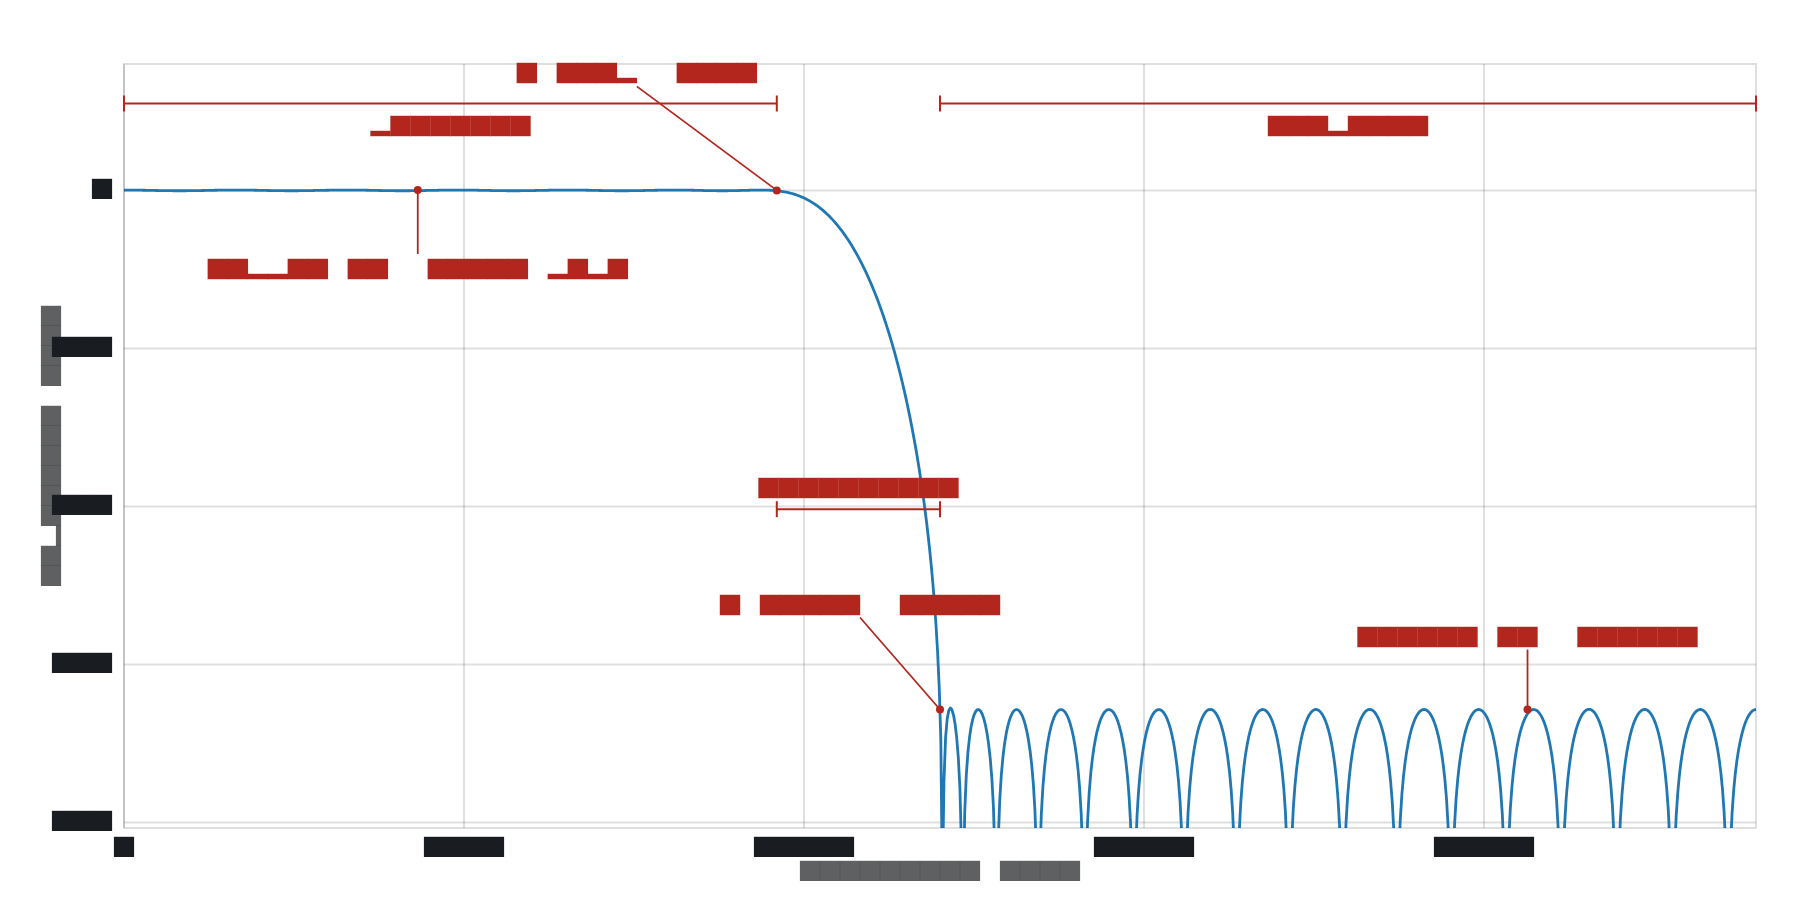
\includegraphics[width=\textwidth]{response-lowpass}
  \caption{A lowpass response, with each parameter named where it acts on the
           curve.}
  \label{fig:lowpass}
\end{figure}

The band edges you type are the ends of the flat regions, \emph{not} the
$-3$\,dB point or the middle of the skirt. The \emph{transition} between them is
empty: nothing is specified there and the design is free to do as it likes,
which is why a narrower transition costs taps.

\begin{itemize}[nosep,leftmargin=*]
  \item \ctl{F stop} of the passband row sets where the passband ends.
  \item \ctl{F start} of the stopband row sets where the stopband begins.
  \item \ctl{Ripple dB} is the peak-to-peak wobble allowed across the passband.
  \item \ctl{Atten.\ dB} is how far down the stopband is held.
\end{itemize}

The ripple is equal across the whole band and the stopband lobes are all the
same height. That is what \emph{equiripple} means, and it is the point of the
Remez exchange: for a given number of taps, no filter has a smaller worst-case
error. The red dots on the curve in the app are the extremal frequencies --- the
points where the error touches its limit.

\subsection{Highpass}

\begin{figure}[htbp]
  \centering
  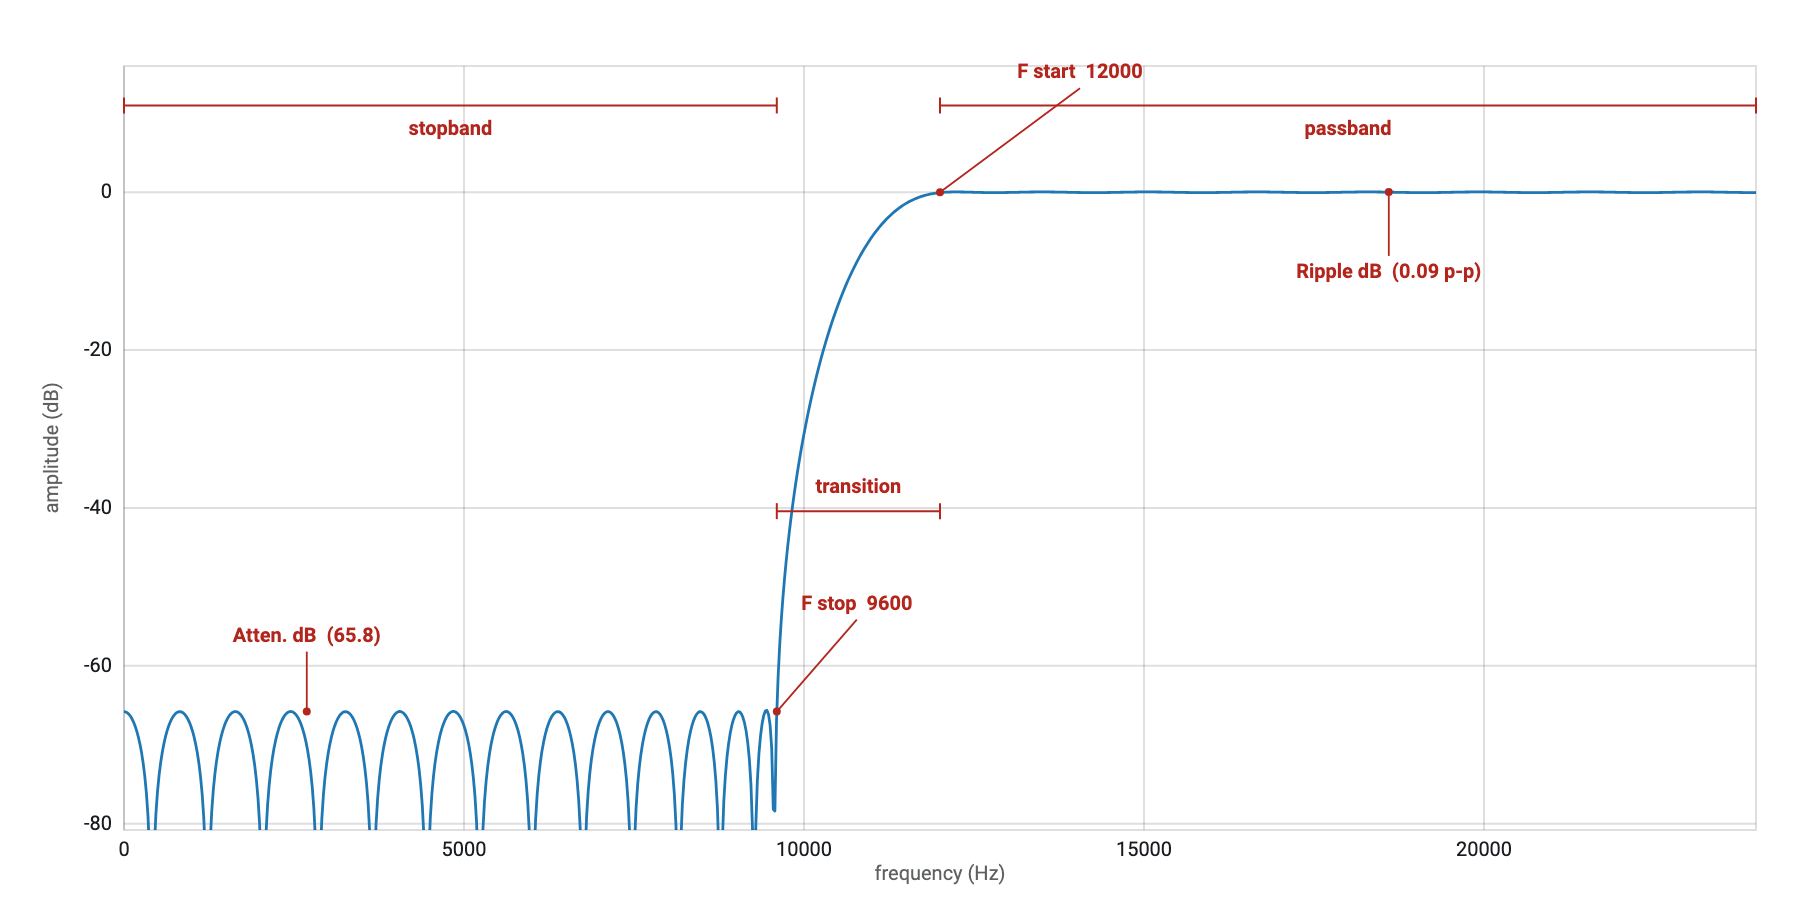
\includegraphics[width=\textwidth]{response-highpass}
  \caption{A highpass. The same picture reflected: the stopband row comes first
           and the passband row second.}
  \label{fig:highpass}
\end{figure}

A highpass wants an \emph{odd} number of taps if it must reach all the way to
Nyquist: an even-length symmetric filter (type II) is forced to zero there and
cannot be a highpass. remez will tell you in the \ctl{Result} panel if you have
asked for something the type cannot do.

\subsection{Bandpass}

\begin{figure}[htbp]
  \centering
  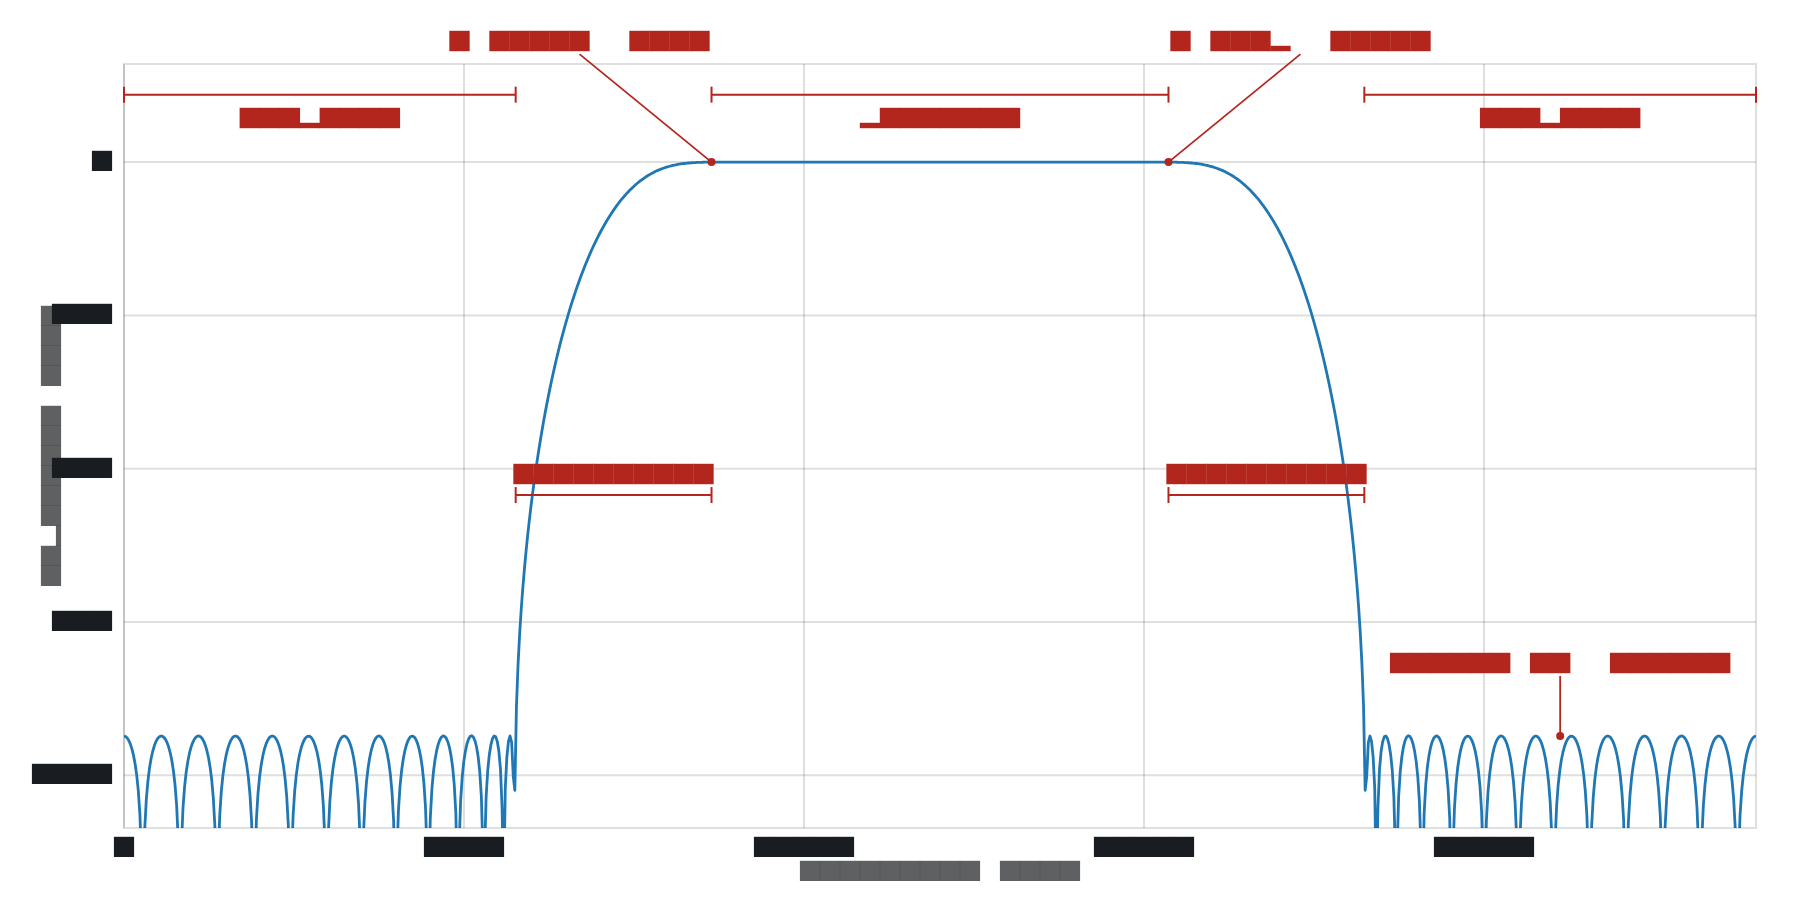
\includegraphics[width=\textwidth]{response-bandpass}
  \caption{A bandpass: three bands, two transitions, and they cost separately
           --- the narrower one sets the taps.}
  \label{fig:bandpass}
\end{figure}

The two stopbands need not have the same attenuation. Give them different
\ctl{Weight} values (or different \ctl{Spec (dB)}) and the exchange will hold
one tighter than the other, spending its taps where you asked.

\clearpage
% ---------------------------------------------------------------------------
\section{The panels, one at a time}

\subsection{Mode}

\begin{figure}[htbp]
  \centering
  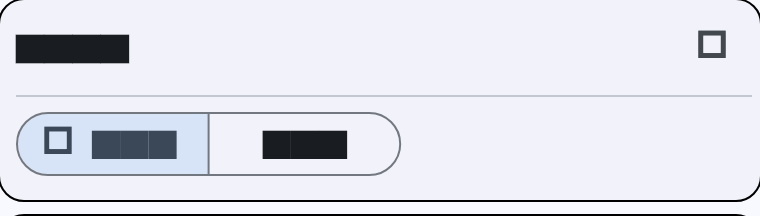
\includegraphics[width=0.62\textwidth]{panel-mode}
  \caption{The Mode panel.}
\end{figure}

FIR or IIR. The two have different \ctl{Filter} and band panels; everything else
is shared. Both designs are kept, so switching back and forth does not lose what
you typed.

\subsection{Filter --- FIR}

\begin{figure}[htbp]
  \centering
  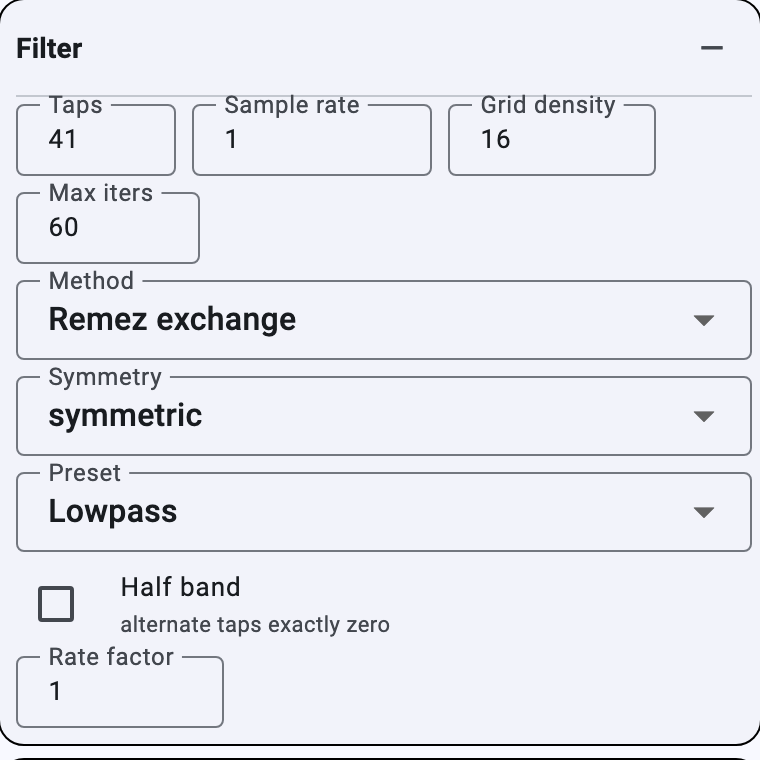
\includegraphics[width=0.62\textwidth]{panel-filter-fir}
  \caption{The FIR Filter panel.}
\end{figure}

\begin{tabularx}{\textwidth}{@{}lY@{}}
  \toprule
  \textbf{field} & \textbf{what it does} \\
  \midrule
  \ctl{Taps} & The filter length $N$. More taps buy a narrower transition or a
    deeper stopband, at a cost of $N$ multiplies and $N-1$ delays per sample. \\
  \addlinespace
  \ctl{Sample rate} & The units everything else is in. Changing it
    \emph{rescales} the band edges so the filter stays the same --- set it
    first, then type edges in Hz. \\
  \addlinespace
  \ctl{Grid density} & How finely the exchange samples each band when it
    searches for the error peaks, in points per coefficient. 16 is the usual
    value. Too coarse and the design steps over a ripple peak and reports a
    smaller $\delta$ than it achieved; see below. \\
  \addlinespace
  \ctl{Max iters} & The iteration cap. 60 is far more than a converging design
    needs; if the \ctl{Result} panel says \emph{did not converge}, the design
    ran out. \\
  \addlinespace
  \ctl{Symmetry} & \lit{symmetric} for ordinary filters; \lit{antisymmetric}
    for a Hilbert transformer or a differentiator, which need a
    90\textdegree{} phase shift. \\
  \addlinespace
  \ctl{Method} & Which algorithm designs the filter: the Remez exchange,
    weighted least squares, or the window method. See
    section~\ref{sec:methods}. \\
  \addlinespace
  \ctl{Window} & Only with the window method: which taper cuts the ideal
    response, and so how deep the stopband gets. \\
  \addlinespace
  \ctl{Kaiser beta} & Only with the Kaiser window, whose attenuation is set by
    this number rather than fixed. \\
  \addlinespace
  \ctl{Preset} & Loads a worked example into the band table. A good starting
    point for a new design. \\
  \addlinespace
  \ctl{Half band} & Design a half-band lowpass: alternate taps come out exactly
    zero, so half the multiplies disappear. See section~\ref{sec:halfband}. \\
  \addlinespace
  \ctl{Passband edge} & Only with \ctl{Half band}: the one edge you get to
    choose. The stopband starts at its mirror about a quarter of the sample
    rate. \\
  \addlinespace
  \ctl{Rate factor} & Split the filter into this many polyphase components, for
    a decimator or an interpolator. 1 means no rate change. \\
  \bottomrule
\end{tabularx}

\paragraph{On grid density.} The reported $\delta$ is a \emph{lower bound} on
the true deviation, never an upper one. Measured on the default lowpass against
the response evaluated at 200\,001 points:

\begin{center}
\begin{tabular}{@{}rrrr@{}}
  \toprule
  \textbf{grid density} & \textbf{reported $\delta$} &
  \textbf{true peak error} & \textbf{optimism} \\
  \midrule
  4              & 0.02848 & 0.03029 & $+6.3\,\%$  \\
  16 (default)   & 0.02877 & 0.02901 & $+0.8\,\%$  \\
  64             & 0.02884 & 0.02886 & $+0.04\,\%$ \\
  \bottomrule
\end{tabular}
\end{center}

Leave it at 16 while exploring; raise it to 64 before you trust the number or
ship the coefficients.

\subsection{Bands and constraints --- FIR}

\begin{figure}[htbp]
  \centering
  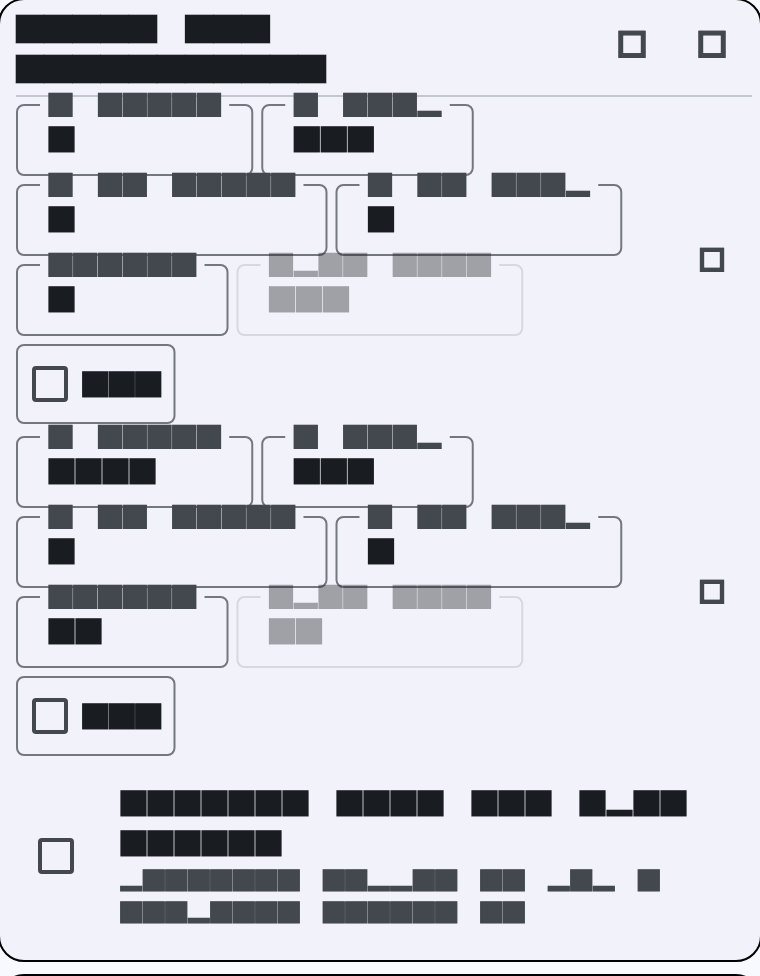
\includegraphics[width=0.62\textwidth]{panel-bands-fir}
  \caption{The FIR band table, one row per band.}
\end{figure}

Bands are given in order and must not overlap; the gaps between them are the
transition regions.

\begin{tabularx}{\textwidth}{@{}lY@{}}
  \toprule
  \textbf{column} & \textbf{what it does} \\
  \midrule
  \ctl{F start}, \ctl{F stop} & The band edges, in the sample-rate units. \\
  \addlinespace
  \ctl{D at start}, \ctl{D at stop} & The desired amplitude at each end. Equal
    for a flat band; different for a sloped one --- a raised-cosine skirt, or a
    differentiator's $2\pi f$. \\
  \addlinespace
  \ctl{Weight} & How hard this band is held relative to the others. The
    exchange equalises $W\,|D-A|$, so doubling a weight halves that band's
    error and spends the taps elsewhere. Only the ratios matter. \\
  \addlinespace
  \ctl{Spec (dB)} & An alternative to \ctl{Weight}, in decibels: peak-to-peak
    ripple for a band with a non-zero target, attenuation for one that targets
    zero. \\
  \addlinespace
  \ctl{1/f} & Weight the band as $w/f$ rather than a constant, which equalises
    \emph{relative} error. What a differentiator needs --- a fixed absolute
    error is negligible at the top of the band and hopeless at the bottom. \\
  \addlinespace
  $\times$ & Remove the row. \\
  \bottomrule
\end{tabularx}

The $\oplus$ button in the panel header adds a band.

\paragraph{Weights from the Spec column.} Tick it and the \ctl{Weight} column
greys out; the weights are derived from the dB figures instead. This is usually
what you want, because ``0.5\,dB ripple and 60\,dB attenuation'' is a
specification and ``weights 1 and 10'' is a guess at one. The \ctl{Result} panel
then checks each band against its spec and, if one is missed, estimates the taps
that would meet it.

\subsection{Filter --- IIR}

\begin{figure}[htbp]
  \centering
  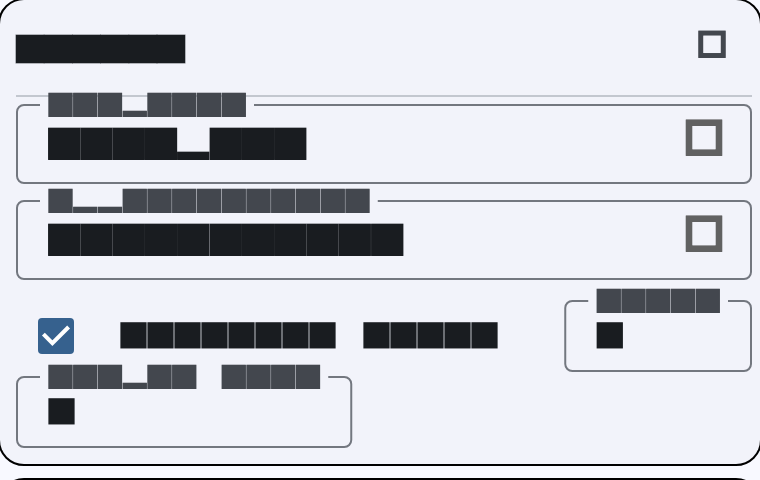
\includegraphics[width=0.62\textwidth]{panel-filter-iir}
  \caption{The IIR Filter panel.}
\end{figure}

\begin{tabularx}{\textwidth}{@{}lY@{}}
  \toprule
  \textbf{field} & \textbf{what it does} \\
  \midrule
  \ctl{Response} & Lowpass, Highpass, Bandpass or Bandstop. Changing it brings
    edge values that make sense for the new shape. \\
  \addlinespace
  \ctl{Approximation} & Butterworth, Chebyshev I, Chebyshev II or Elliptic;
    see section~\ref{sec:approximations}. \\
  \addlinespace
  \ctl{Order} & The prototype order. The digital filter has twice this many
    poles for a bandpass or bandstop. \\
  \addlinespace
  \ctl{Smallest order} & Let remez pick the lowest order that meets the
    specification. Usually leave this on; turn it off to explore what a
    particular order does. \\
  \bottomrule
\end{tabularx}

\subsection{Bands and specification --- IIR}

\begin{figure}[htbp]
  \centering
  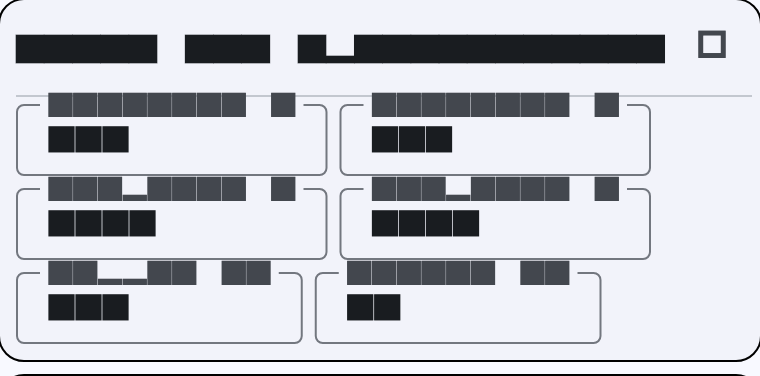
\includegraphics[width=0.72\textwidth]{panel-bands-iir}
  \caption{The IIR band panel: edges and tolerances rather than a table.}
\end{figure}

\begin{tabularx}{\textwidth}{@{}lY@{}}
  \toprule
  \textbf{field} & \textbf{what it does} \\
  \midrule
  \ctl{Passband} (1, 2) & Where the passband ends. Two fields for a bandpass or
    bandstop. \\
  \addlinespace
  \ctl{Stopband} (1, 2) & Where the stopband begins. \\
  \addlinespace
  \ctl{Ripple dB} & Peak-to-peak passband ripple. Butterworth has no ripple by
    construction, but the figure is still used: the prototype is widened so the
    response is exactly this far down at the passband edge, rather than at the
    conventional $-3$\,dB point. That puts all four approximations on the same
    footing. \\
  \addlinespace
  \ctl{Atten.\ dB} & Required stopband attenuation. \\
  \bottomrule
\end{tabularx}

The design places the edge that its approximation actually pins down: the
passband edge for Butterworth, Chebyshev I and elliptic, the stopband edge for
Chebyshev II. The other edge falls where the order puts it.

\subsection{Arithmetic}

\begin{figure}[htbp]
  \centering
  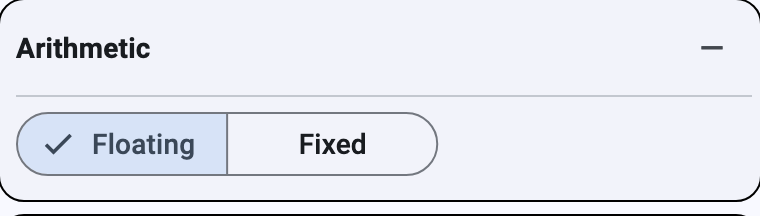
\includegraphics[width=0.62\textwidth]{panel-arithmetic}
  \caption{In floating point the coefficients are doubles and the plots show
           the ideal design.}
\end{figure}

Switch to \ctl{Fixed} and remez quantizes the coefficients and re-analyses, so
the plots and the report show the filter you would actually build.

\begin{figure}[htbp]
  \centering
  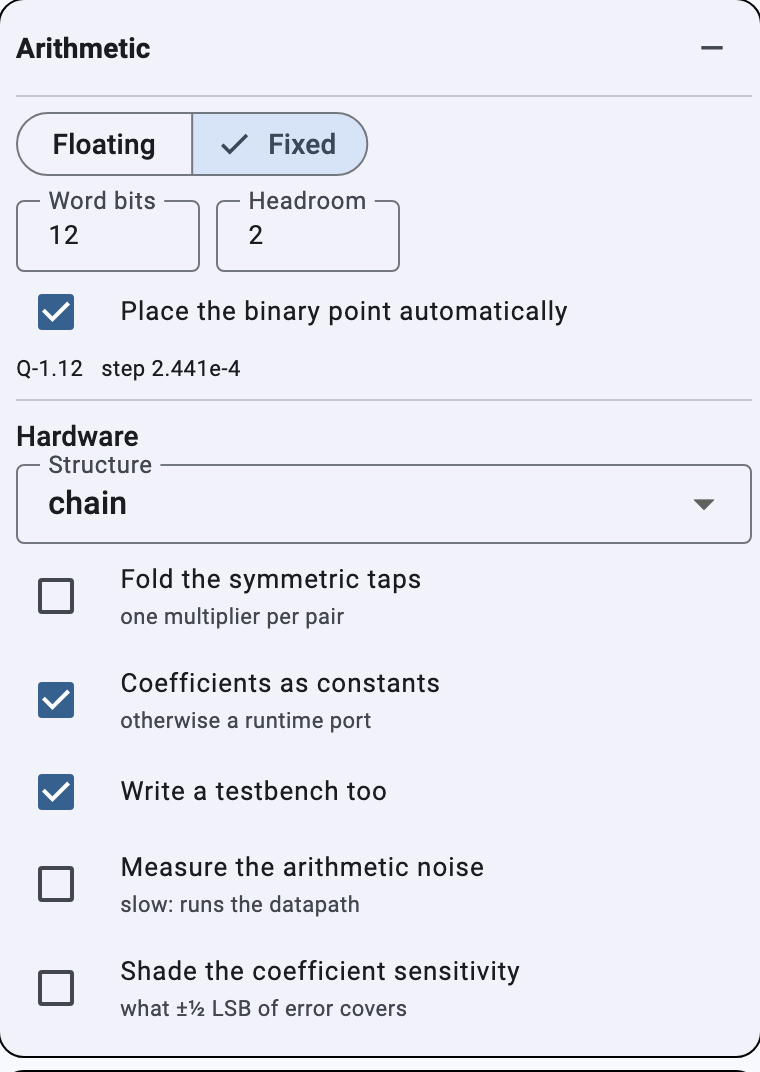
\includegraphics[width=0.55\textwidth]{panel-arithmetic-fixed}
  \caption{In fixed point the word length and the hardware options appear.}
\end{figure}

\begin{tabularx}{\textwidth}{@{}lY@{}}
  \toprule
  \textbf{field} & \textbf{what it does} \\
  \midrule
  \ctl{Word bits} & Coefficient word length. \\
  \addlinespace
  \ctl{Headroom} & Extra integer bits in the datapath, above the coefficient
    format. This is what keeps the adders off their limits; 2 is a sensible
    default. \\
  \addlinespace
  \ctl{Place the binary point automatically} & Puts the binary point where the
    largest coefficient just fits. Turn it off to set the fraction length
    yourself. \\
  \addlinespace
  \ctl{Structure} & How the multiplies are summed in hardware: \lit{chain} (one
    adder per tap --- smallest, slowest), \lit{tree} (balanced, registered
    between levels --- fastest), \lit{mac} (one multiplier reused, one term per
    clock --- smallest of all, one sample per $N$ clocks). \\
  \addlinespace
  \ctl{Fold the symmetric taps} & A linear-phase filter has equal taps in
    pairs, so one pre-add plus one multiply serves two of them. Roughly halves
    the multipliers. \\
  \addlinespace
  \ctl{Coefficients as constants} & Compile them into the RTL so synthesis can
    specialise each multiplier. Turn it off for a runtime coefficient port. \\
  \addlinespace
  \ctl{Write a testbench too} & Emit a self-checking testbench beside the RTL.
    It carries the expected output of every sample, so running it proves the
    hardware matches the plots. \\
  \bottomrule
\end{tabularx}

The line under the fields reports the Q format, the step size, and a warning if
any coefficient saturated. A saturated coefficient means the hardware is not the
filter you designed --- give it more bits.

The last two boxes are analyses rather than build options, and both cost real
time, which is why they are off by default.

\paragraph{Measure the arithmetic noise.} Rounding the coefficients is only half
of what fixed point does to a filter; the other half is that every product and
every sum is rounded too. This drives the exact integer datapath --- the one the
RTL export would generate, structure and folding included --- with a few
thousand samples, compares its output against the same filter computed exactly,
and takes the spectrum of the difference. That level is drawn on the magnitude
plot as a dashed line, and the \ctl{Result} panel says what it means: a stopband
below the line is a number on a plot rather than a filter you can build.

\paragraph{Shade the coefficient sensitivity.} Nudges every coefficient
independently by up to half an LSB, a hundred and twenty-odd times, and shades
the region the responses cover. A thin band means the design has margin. A band
that swallows the stopband means the filter only works at the exact values it
was given. For an IIR it also counts the draws that came out unstable, which is
the failure that rounding a high-order elliptic design really produces.

\subsection{File}

\begin{figure}[htbp]
  \centering
  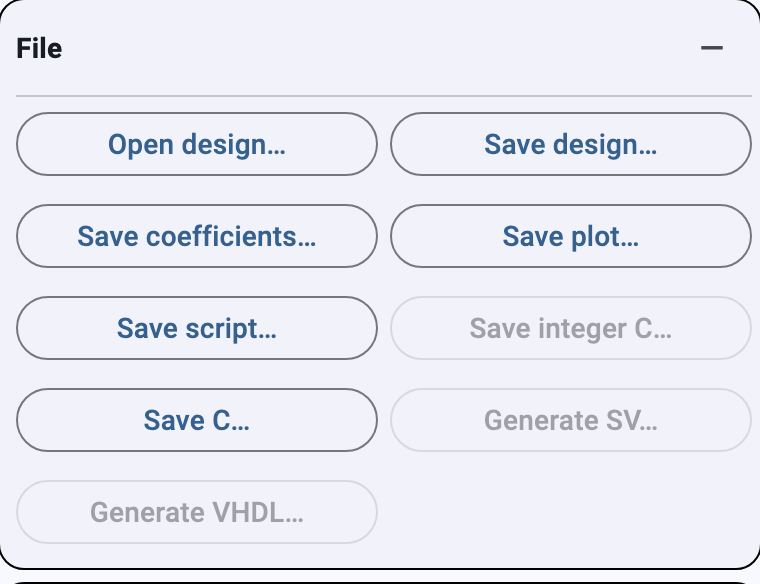
\includegraphics[width=0.62\textwidth]{panel-file}
  \caption{The File panel.}
\end{figure}

\begin{tabularx}{\textwidth}{@{}lY@{}}
  \toprule
  \textbf{button} & \textbf{what it writes} \\
  \midrule
  \ctl{Open design\dots} & Reads a \lit{.remz} (or an older \lit{.json})
    design. \\
  \addlinespace
  \ctl{Save design\dots} & Writes the whole specification as \lit{.remz}; see
    section~\ref{sec:savefile}. \\
  \addlinespace
  \ctl{Save coefficients\dots} & The coefficients alone. A \lit{.h} extension
    gets C arrays; anything else gets CSV with a commented header. In fixed
    point both carry the stored integers alongside the rounded values. \\
  \addlinespace
  \ctl{Save plot\dots} & The right-hand pane as a PNG --- whichever view is
    showing, in whichever theme, at twice screen resolution. \\
  \addlinespace
  \ctl{Save C\dots} & One self-contained C file: a library
    (\lit{init\_filter} / \lit{process\_sample} / \lit{free\_filter}) and a
    program that filters raw 64-bit floats from stdin to stdout. \\
  \addlinespace
  \ctl{Save script\dots} & A NumPy module or a MATLAB function, chosen by the
    extension you give it --- \lit{.py} or \lit{.m}. Both define the
    coefficients and call the library routine; an FIR goes to
    \lit{lfilter}/\lit{filter}, a cascade to \lit{sosfilt}. \\
  \addlinespace
  \ctl{Save integer C\dots} & The same filter with no floating point anywhere:
    signed integers, products rounded and saturated, sums saturated, in the
    order the chosen structure sums them. It is the \emph{same} arithmetic as
    the generated RTL, bit for bit, which makes it the reference model to run on
    the target before the hardware exists. Needs fixed point. \\
  \addlinespace
  \ctl{Generate SV\dots}, \ctl{Generate VHDL\dots} & Synthesisable RTL for the
    structure chosen in \ctl{Arithmetic}, with its testbench. Both need
    fixed-point coefficients; until then they are disabled and the tooltip says
    why. \\
  \bottomrule
\end{tabularx}

\subsection{Display}

\begin{figure}[htbp]
  \centering
  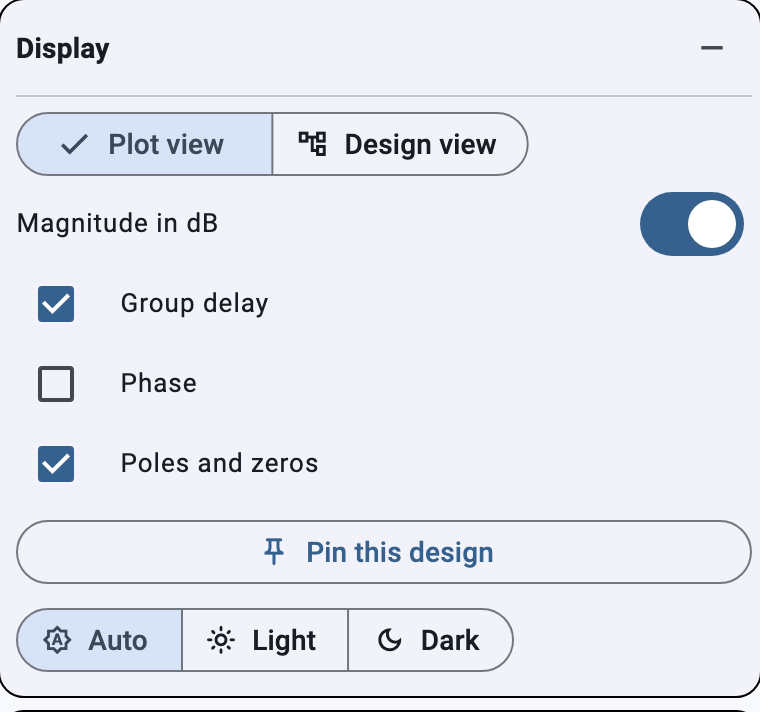
\includegraphics[width=0.62\textwidth]{panel-display}
  \caption{The Display panel.}
\end{figure}

\ctl{Plot view} is the response plots. \ctl{Design view} draws the filter
as the thing you would build --- the adders, delays and multipliers, each
labelled with its actual constant. \ctl{Magnitude in dB} switches the top plot
between decibels and linear amplitude. \ctl{Auto\,/\,Light\,/\,Dark} follows the
desktop or forces a theme; the saved plot uses whichever is showing.

Three checkboxes choose which of the optional plots are drawn:

\begin{itemize}[leftmargin=*]
  \item \ctl{Group delay} --- how many samples each frequency is held up by. A
        linear-phase FIR draws a flat line at $(N-1)/2$, which is the claim
        being made for it, verified rather than asserted. An IIR does not: its
        delay peaks around the band edges, and that peak is the price of the
        coefficients it saved.
  \item \ctl{Phase} --- the same information one integral earlier, unwrapped.
        Off by default because group delay says it more directly. The steps of
        180\textdegree{} in an FIR's phase are its zeros on the unit circle.
  \item \ctl{Poles and zeros} --- the $z$ plane, with the unit circle drawn.
        Every pole inside it or the filter is unstable, and in fixed point the
        design's poles and the poles the \emph{rounded} coefficients actually
        give are drawn together, so a pole that rounding has pushed onto the
        circle is something you see rather than something you infer from a
        magnitude plot behaving oddly.
\end{itemize}

\ctl{Pin this design} keeps the current response on the axes, dashed, while you
edit another against it --- the way to answer ``is 61 taps really buying me
anything here?'' without alt-tabbing between screenshots. The button turns into
\ctl{Unpin} and names what it is holding.

The two arrows in the title bar are undo and redo, on \lit{Cmd-Z} and
\lit{Shift-Cmd-Z}. They step through complete designs, not individual
keystrokes, and reach everything the save file reaches.

\subsection{Signal}

Push a test signal through the filter and plot what came out, alongside what
went in. The response plots say what happens to a sine wave of every frequency,
one at a time and forever; that is the complete answer and it is not always the
legible one.

\begin{tabularx}{\textwidth}{@{}lY@{}}
  \toprule
  \textbf{signal} & \textbf{what it is for} \\
  \midrule
  \ctl{impulse} & the taps themselves \\
  \ctl{step} & overshoot, ringing, and the pre-echo linear phase pays for its
    symmetry \\
  \ctl{chirp} & the whole band swept, so the transition is a fade you can point
    at \\
  \ctl{tone} & one frequency, for gain and delay \\
  \ctl{noise} & everything at once, for the noise floor \\
  \ctl{square} & harmonics, and what happens to the ones the filter removes \\
  \bottomrule
\end{tabularx}

In fixed point it runs the signal twice: once through the design in double
precision and once through the exact integer datapath. Both are drawn, and the
title reports the difference between them and how many samples the datapath had
to clip. Clipping is not rounding that averages away --- it is the filter
ceasing to be linear --- so one clipped sample is a headroom problem, not a
word-length one.

\subsection{Result}

\begin{figure}[htbp]
  \centering
  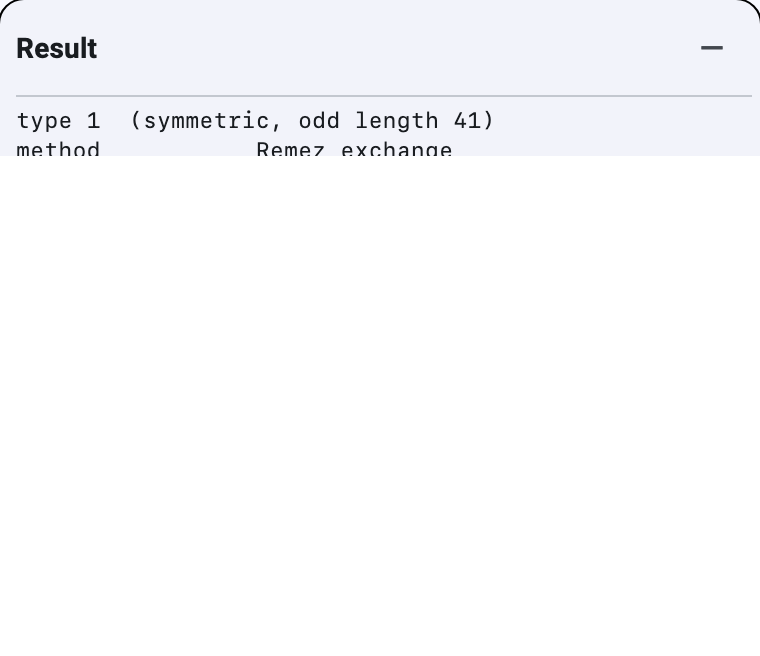
\includegraphics[width=0.62\textwidth]{panel-result}
  \caption{The report: what was designed, and how well.}
\end{figure}

Filter type and length, iterations, the weighted $\delta$, then a table of each
band's achieved deviation in both linear and dB terms. In fixed point it adds
the Q format, the worst rounding error and the datapath width; with \ctl{Weights
from the Spec column} on it adds a spec check per band. It ends with the filter
itself --- the taps for an FIR, the second-order sections for an IIR --- which
you can select and copy.

\clearpage
% ---------------------------------------------------------------------------
\section{Filter types and what they are good for}

\subsection{The four linear-phase FIR types}

Symmetry and length together decide what a filter can do. remez picks the type
for you and names it in the report; the constraints are not arbitrary but come
from what the amplitude response is forced to be at DC and at Nyquist.

\begin{center}
\begin{tabular}{@{}clccc>{\raggedright\arraybackslash}p{45mm}@{}}
  \toprule
  \textbf{type} & \textbf{symmetry} & \textbf{length} &
  \textbf{zero at DC?} & \textbf{zero at Nyq.?} & \textbf{use for} \\
  \midrule
  I   & symmetric     & odd  & no  & no  & anything: lowpass, highpass,
                                            bandpass, bandstop, multiband \\
  \addlinespace
  II  & symmetric     & even & no  & \textbf{forced} & lowpass and bandpass
                                            only; never a highpass \\
  \addlinespace
  III & antisymmetric & odd  & \textbf{forced} & \textbf{forced} & Hilbert
                                            transformers, differentiators \\
  \addlinespace
  IV  & antisymmetric & even & \textbf{forced} & no & differentiators,
                                            antisymmetric highpass work \\
  \bottomrule
\end{tabular}
\end{center}

Practically: leave \ctl{Symmetry} on \lit{symmetric} and use an odd number of
taps unless you have a reason not to. Choose \lit{antisymmetric} when you want a
90\textdegree{} phase shift --- the Hilbert transformer and differentiator
presets set it for you.

\subsection{Three ways to design an FIR}
\label{sec:methods}

The \ctl{Method} pulldown offers three, and they are not ranked: each minimises
something different, and which one is right depends on what your specification
actually means.

\begin{tabularx}{\textwidth}{@{}lllc@{}}
  \toprule
  \textbf{method} & \textbf{minimises} & \textbf{the stopband it gives}
    & \textbf{iterates?} \\
  \midrule
  Remez exchange & the \emph{worst} weighted error
    & one flat wall of equal lobes & yes \\
  least squares & the \emph{total} squared error
    & worst at the transition, quieter out & no \\
  window & nothing & whatever the window's sidelobes are & no \\
  \bottomrule
\end{tabularx}

\paragraph{The exchange} is the default because a specification is usually a
limit that must not be exceeded, and minimax is exactly the promise ``nowhere
worse than this''. For a given number of taps no filter has a smaller worst-case
error.

\paragraph{Least squares} gives that up and buys total energy instead. Its error
is largest at the band edges and falls away from them, so the far stopband ends
up much deeper than an equiripple design would put it. Reach for it when the
thing being rejected is broadband, or when the filter feeds something that
integrates: holding a corner nobody is standing on is taps spent for nothing.

\paragraph{The window method} does not optimise at all. It takes the exact
impulse response of the ideal brick wall, which is infinitely long, cuts it to
length, and tapers the cut so the truncation does not ring. Two things recommend
it: there is no iteration to fail to converge, and the stopband depth is a
property of the window rather than of the design.

\begin{tabularx}{\textwidth}{@{}llY@{}}
  \toprule
  \textbf{window} & \textbf{sidelobes} & \textbf{notes} \\
  \midrule
  rectangular & ${\approx}21$\,dB & no taper at all; the ringing is the point of
    comparison \\
  Hann & ${\approx}44$\,dB & sidelobes fall away fastest, so the far stopband is
    the best of the fixed three \\
  Hamming & ${\approx}53$\,dB & lowest \emph{first} sidelobe, but it rolls off
    slowly \\
  Blackman & ${\approx}74$\,dB & the deepest, and the widest main lobe, so it
    needs the longest filter \\
  Kaiser & set by $\beta$ & the adjustable one: $\beta$ trades transition width
    against depth \\
  \bottomrule
\end{tabularx}

The catch is the other direction. A window only \emph{reaches} its figure once
the filter is long enough for the window's main lobe to fit inside the
transition. Ask for a narrow transition with a Blackman window and a short
filter and you get neither: 161 taps across this document's example transition
reaches $-75$\,dB, and 81 taps manages only $-39$\,dB.

\subsection{Half band and polyphase}
\label{sec:halfband}

Two ways of not doing arithmetic you do not have to do.

\paragraph{A half-band lowpass} has every other tap at exactly zero. That is not
a trick played on an ordinary design --- it falls out of the problem. Ask for a
filter that is 1 up to $f_p$ and 0 from $f_s/2 - f_p$, with the two bands
weighted \emph{equally}, and the answer satisfies
\[
  A(\omega) + A(\pi - \omega) = 1
\]
identically: if it did not, averaging it with its own mirror would give an
equally good filter, and the minimax solution is unique. Written out in taps,
that identity says the centre tap is $\tfrac12$ and every tap an even number of
places from it is zero. So ticking \ctl{Half band} does not post-process
anything. It constrains: one band edge instead of a table, equal weights, and a
length rounded to the nearest $4k+3$, because those are the conditions under
which the answer is a half-band filter at all. The exchange then leaves the
vanishing taps at about $10^{-16}$, and the program sets them to the zero they
mathematically are. A 43-tap half band needs 23 multiplies instead of 43, and
the \ctl{Result} panel says so.

\paragraph{A polyphase decomposition} is what makes a rate change cost what it
should. Decimating by $M$ throws away $M-1$ of every $M$ outputs, so computing
them was wasted; splitting the filter into $M$ sub-filters, each fed every $M$th
sample, and summing them computes only the outputs that survive. Interpolating
by $L$ is the mirror image. Either way the multiplies per sample fall by the
rate factor and \emph{no arithmetic changes} --- the output is the same to the
last bit. Set \ctl{Rate factor} above 1 and the phases appear in the
\ctl{Result} panel and in the saved coefficients, as \lit{e0}, \lit{e1},
\dots{} where phase $p$ holds taps $p$, $p+M$, $p+2M$ and so on.

\subsection{FIR against IIR}

\begin{center}
\begin{tabularx}{\textwidth}{@{}lYY@{}}
  \toprule
  & \textbf{FIR} & \textbf{IIR} \\
  \midrule
  phase & exactly linear & not linear; group delay varies, worst near the band
    edges \\
  \addlinespace
  stability & unconditional & must be checked; remez reports
    $\max|p|$ \\
  \addlinespace
  coefficients for a sharp filter & many (tens to hundreds) & few (a handful of
    biquads) \\
  \addlinespace
  quantization & graceful; the response degrades smoothly & poles can move onto
    or outside the unit circle \\
  \addlinespace
  transient & finite, $N$ samples & infinite \\
  \bottomrule
\end{tabularx}
\end{center}

Reach for FIR when phase matters, when the filter must be provably stable, or
when it will run on hardware with multipliers to spare. Reach for IIR when you
need a sharp filter cheaply and phase is not critical --- audio equalisation,
control loops, decimation front-ends.

\subsection{The four IIR approximations}
\label{sec:approximations}

Everything gives up something to get selectivity.

\begin{center}
\begin{tabular}{@{}lllcl@{}}
  \toprule
  & \textbf{passband} & \textbf{stopband} &
  \textbf{selectivity} & \textbf{phase} \\
  \midrule
  \textbf{Butterworth}  & maximally flat & monotonic  & worst  & best behaved \\
  \textbf{Chebyshev I}  & equiripple     & monotonic  & better & worse \\
  \textbf{Chebyshev II} & monotonic      & equiripple & better & worse \\
  \textbf{Elliptic}     & equiripple     & equiripple & best   & worst \\
  \bottomrule
\end{tabular}
\end{center}

\begin{description}[leftmargin=*,style=nextline]
  \item[Butterworth] When the passband must be flat and you can afford the
    order. No ripple anywhere; the roll-off is gentle.
  \item[Chebyshev I] Accept some passband ripple, get a steeper skirt. The
    ripple is equal across the whole passband.
  \item[Chebyshev II] The mirror: a clean passband and an equiripple stopband
    with transmission zeros in it. Useful when passband flatness matters more
    than stopband uniformity, and it has the gentlest phase of the two
    Chebyshevs.
  \item[Elliptic (Cauer)] Ripple in both bands, and the steepest transition any
    order can give. The order equation is a three-way trade: you cannot ask for
    order, ripple \emph{and} transition width independently, since any two fix
    the third. Use it when you want the cheapest filter that meets a hard mask,
    and avoid it when phase or transient response matters.
\end{description}

With \ctl{Smallest order} ticked, remez tells you the lowest order that meets
your specification. The \ctl{Result} panel reports both the order used and the
estimate, so you can see how much margin you have.

\clearpage
% ---------------------------------------------------------------------------
\section{The save file}
\label{sec:savefile}

\ctl{Save design\dots} writes a \lit{.remz} file. It is UTF-8 JSON --- the
extension only changes what the desktop does with it, and anything that reads
JSON still can. macOS declares it as \lit{com.deadhat.remez.design} conforming
to \lit{public.json}, so a double-clicked design opens in remez.

The file records the \emph{specification}, not the result: the coefficients are
not in it, because opening the file redesigns the filter from the numbers you
typed. That keeps a design portable between versions, and between this program
and the Python prototype in \lit{python\_prototype/}, which reads and writes the
same format.

\subsection{A complete example}

{\footnotesize
\begin{verbatim}
{
  "format": "remez-filter-design",
  "version": 1,
  "mode": "FIR — Remez exchange",
  "fs": 48000.0,
  "fir": {
    "numtaps": 41,
    "symmetry": "symmetric",
    "grid_density": 16,
    "maxiter": 60,
    "use_spec": false,
    "method": "remez",
    "window": "hamming",
    "kaiser_beta": "8.6",
    "half_band": false,
    "half_band_edge": "0.2",
    "rate_factor": 1,
    "rate_change": "decimate",
    "bands": [
      [
        0.0,
        0.2,
        1.0,
        1.0,
        1.0,
        0.5,
        false
      ],
      [
        0.25,
        0.5,
        0.0,
        0.0,
        10.0,
        50.0,
        false
      ]
    ]
  },
  "iir": {
    "response": "Lowpass",
    "approximation": "Butterworth",
    "order": 6,
    "auto_order": true,
    "wp": [
      "0.2",
      "0.4"
    ],
    "ws": [
      "0.3",
      "0.45"
    ],
    "rp": "0.5",
    "rs": "40"
  },
  "arithmetic": {
    "kind": "fixed",
    "word_bits": 16,
    "auto_frac": true,
    "frac_bits": -611,
    "headroom": 2,
    "fixed_coeffs": true,
    "structure": "tree",
    "folded": false,
    "testbench": true,
    "measure_noise": false,
    "sensitivity": false
  },
  "display": {
    "log_scale": true,
    "view": "Plot view",
    "appearance": "system",
    "phase": false,
    "signal": false,
    "signal_kind": "chirp",
    "signal_frequency": "0.05",
    "signal_length": 512,
    "group_delay": true,
    "zplane": true
  }
}
\end{verbatim}
}

\emph{Note:} the \lit{mode} value contains an em dash in the real file
(\lit{"FIR}~---~\lit{Remez exchange"}); it is written as a hyphen above only so
this listing stays plain ASCII.

\subsection{Semantics}

\paragraph{Top level.}\mbox{}

\begin{tabularx}{\textwidth}{@{}lY@{}}
  \toprule
  \textbf{key} & \textbf{meaning} \\
  \midrule
  \lit{format} & Must be \lit{"remez-filter-design"}. A file without it is
    rejected. \\
  \lit{version} & Currently \lit{1}. \\
  \lit{mode} & \lit{"FIR --- Remez exchange"} or \lit{"IIR --- bilinear
    transform"}. Only the leading \lit{FIR}/\lit{IIR} is significant to the
    reader. \\
  \lit{fs} & Sample rate. \textbf{Every frequency in the file is in these
    units} --- the file does not normalise. \\
  \bottomrule
\end{tabularx}

Both the \lit{fir} and \lit{iir} sections are always written, whichever mode is
active, so switching mode after loading finds the other design where you left
it.

\paragraph{\lit{fir}.} \lit{bands} is an array of rows, each a fixed
seven-element array:

\begin{center}
\begin{tabular}{@{}cccccccc@{}}
  \toprule
  index & 0 & 1 & 2 & 3 & 4 & 5 & 6 \\
  \midrule
  field & \lit{f\_start} & \lit{f\_stop} & \lit{d\_start} & \lit{d\_stop}
        & \lit{weight} & \lit{spec\_dB} & \lit{inverse\_f} \\
  \bottomrule
\end{tabular}
\end{center}

The first five and the seventh are what the table shows; \lit{spec\_dB} is used
in place of \lit{weight} when \lit{use\_spec} is true. \lit{inverse\_f} is a
boolean. \lit{grid\_density} and \lit{maxiter} are the search parameters
described above, and \lit{symmetry} is \lit{"symmetric"} or
\lit{"antisymmetric"}.

\begin{sloppypar}
\lit{method} is \lit{"remez"}, \lit{"leastSquares"} or \lit{"window"};
\lit{window} is \lit{"rectangular"}, \lit{"hann"}, \lit{"hamming"},
\lit{"blackman"} or \lit{"kaiser"}, and \lit{kaiser\_beta} is a string.
\lit{half\_band} is a boolean and \lit{half\_band\_edge} the one edge it needs.
\lit{rate\_factor} is an integer, 1 for no rate change, and \lit{rate\_change}
is \lit{"decimate"} or \lit{"interpolate"}.
\end{sloppypar}

\paragraph{\lit{iir}.} \lit{response} and \lit{approximation} are stored as the
\emph{display} spellings --- \lit{"Lowpass"}, \lit{"Chebyshev I"} --- because
that is what the Python prototype writes. The reader accepts either those or the
internal keys (\lit{lowpass}, \lit{chebyshev1}).

\lit{wp} and \lit{ws} are arrays of two edge values as strings, even for a
lowpass, where only the first is used. \lit{rp} and \lit{rs} are the ripple and
attenuation in dB. \lit{order} applies when \lit{auto\_order} is false.

\paragraph{\lit{arithmetic}.} \lit{kind} is \lit{"float"} or \lit{"fixed"}. The
rest are the Arithmetic panel's fields: \lit{word\_bits}, \lit{auto\_frac},
\lit{frac\_bits}, \lit{headroom}, and the hardware options \lit{fixed\_coeffs},
\lit{structure} (\lit{"chain"}, \lit{"tree"} or \lit{"mac"}), \lit{folded} and
\lit{testbench}. \lit{measure\_noise} and \lit{sensitivity} switch on the two
analyses.

\paragraph{\lit{display}.} \lit{log\_scale}, \lit{view} (\lit{"Plot view"} or
\lit{"Design view"}) and \lit{appearance} (\lit{"system"}, \lit{"light"} or
\lit{"dark"}), plus which optional plots are drawn --- \lit{phase},
\lit{group\_delay} and \lit{zplane}, all booleans --- and the signal runner's
\lit{signal}, \lit{signal\_kind} (\lit{"impulse"}, \lit{"step"}, \lit{"chirp"},
\lit{"tone"}, \lit{"noise"} or \lit{"square"}), \lit{signal\_frequency} and
\lit{signal\_length}. Of those, only \lit{log\_scale} and \lit{view} are keys
the Python prototype writes.

\subsection{Compatibility}

Reading is deliberately forgiving.

\begin{itemize}[leftmargin=*]
  \item \textbf{Anything missing keeps its current value.} A file with only
        \lit{format} and \lit{version} loads and changes nothing.
  \item \textbf{Anything unrecognised is preserved.} The Python prototype
        writes \lit{show\_ext}, \lit{show\_noise}, \lit{show\_spec} and
        \lit{folded\_panels}, which this program has no controls for. They are
        carried through a load-and-save round trip rather than dropped, so
        editing a design here does not strip settings the other program relies
        on. \lit{appearance} is this program's own addition and the Python's
        reader ignores it in the same way.
  \item \textbf{A file that is not a design is refused} rather than
        half-loaded.
\end{itemize}

\vfill
\noindent\rule{\textwidth}{0.4pt}\\
{\small Figures generated by \lit{test/make\_docs\_test.dart}; rerun it with
\lit{-{}-update-goldens} after changing the interface.}

\end{document}
